\documentclass{article}

% if you need to pass options to natbib, use, e.g.:
% \PassOptionsToPackage{numbers, compress}{natbib}
% before loading nips_2018

% ready for submission
\usepackage[final, nonatbib]{nips_2018}
\usepackage{graphicx}
\usepackage[font=small,labelfont=bf]{caption}

% to compile a preprint version, e.g., for submission to arXiv, add
% add the [preprint] option:
% \usepackage[preprint]{nips_2018}

% to compile a camera-ready version, add the [final] option, e.g.:
% \usepackage[final]{nips_2018}

% to avoid loading the natbib package, add option nonatbib:
% \usepackage[nonatbib]{nips_2018}

\usepackage[utf8]{inputenc} % allow utf-8 input
\usepackage[T1]{fontenc}    % use 8-bit T1 fonts
\usepackage{hyperref}       % hyperlinks
\usepackage{url}            % simple URL typesetting
\usepackage{booktabs}       % professional-quality tables
\usepackage{amsfonts}       % blackboard math symbols
\usepackage{nicefrac}       % compact symbols for 1/2, etc.
\usepackage{microtype}      % microtypography
\usepackage[backend=biber, style=numeric, sorting=none]{biblatex}
\addbibresource{ref.bib}

\newcommand{\beginsupplement}{%
        \renewcommand{\thetable}{S\arabic{table}}%
        \renewcommand{\thefigure}{S\arabic{figure}}%
}

\title{\large{Classifying alignments from duplicated genomic sequence}}

% The \author macro works with any number of authors. There are two
% commands used to separate the names and addresses of multiple
% authors: \And and \AND.
%
% Using \And between authors leaves it to LaTeX to determine where to
% break the lines. Using \AND forces a line break at that point. So,
% if LaTeX puts 3 of 4 authors names on the first line, and the last
% on the second line, try using \AND instead of \And before the third
% author name.

\author{
  Mitchell R. Vollger
  %\thanks{Use footnote for providing further
   % information about author (webpage, alternative
    %address)---\emph{not} for acknowledging funding agencies.} 
    \\
  Department of Genome Sciences\\
  University of Washington\\
  \texttt{mvollger@uw.edu} \\
  %% examples of more authors
  %% \And
  %% Coauthor \\
  %% Affiliation \\
  %% Address \\
  %% \texttt{email} \\
  %% \AND
  %% Coauthor \\
  %% Affiliation \\
  %% Address \\
  %% \texttt{email} \\
  %% \And
  %% Coauthor \\
  %% Affiliation \\
  %% Address \\
  %% \texttt{email} \\
  %% \And
  %% Coauthor \\
  %% Affiliation \\
  %% Address \\
  %% \texttt{email} \\
}

\begin{document}
% \nipsfinalcopy is no longer used

\maketitle
%%%%-------------------------------------------%%%%%
%%%% FROM ABOVE HERE CAN USE FOR FINAL PROJECT %%%%%
%%%%-------------------------------------------%%%%%

\section*{Introduction}

Mammalian genomes contain long stretches of duplicated sequence that is nearly identical and often spanning more than 100,000 bases \parencite{Lander2001, Waterston2002}. These stretches of high sequence identity are not possible to resolve using common sequencing and assembly strategies because alignments between overlapping DNA sequences in these regions could possibly represent DNA sequences that originate from disparate copies of the duplication \parencite{Pop2004, Chin2016, Gordon2016, Koren2017}. Previous work \parencite{Chaisson2017, Vollger2018} proposed a method for assembling these sequences; however, this method only produces "local" assemblies of duplications that are not ordered and oriented within the context of the rest of the genome assembly.

A goal of my research is to use ultra-long sequencing data \parencite{Jain2018} to order and orient "local" assemblies of duplications in the context of additional genomic sequence. However, before this can be accomplished the alignments between the local assemblies and ultra-long reads need to be classified as either: alignments that are between disparate copies of a duplication (i.e. false alignments), or alignments representing overlaps between the same copy of the duplication (i.e. true alignments). Filtering alignments based on simple statistics such as the percent identity of the alignment has proved insufficient to classify these as true or false alignments (\autoref{fig:LHR}). 

\section*{Data}
Using ultra-long sequencing data \parencite{Jain2018} and an internal ultra-long sequencing data I have generated a data set representing alignments between local assemblies of duplications and ultra-long sequencing data.\\
\texttt{https://eichlerlab.gs.washington.edu/help/mvollger/CSE546/OntToSDA.nof.bam.tsv} \\
To create labels for the data set I have aligned both the local assemblies and ultra-long sequencing data to the human reference (which has these regions correctly assembled) and determined whether the alignments I observed in my data set are reflected in the human reference. Combining these I have available to me 4,801 alignments each with true/false labels. The classes are not equally represented, with only 1/5 of alignments classified as true.   

\section*{Preliminary Results and Methods}
For the milestone I have applied three classification techniques to the data, SVM \parencite{Hastie2008}, Random Forests \parencite{Ho1995, Breiman2001}, and Gradient Boosting \parencite{Friedman1999GreedyMachine}. \parencite{Pedregosa2011Scikit-learnPython} Before applying these methods to my data, I performed several additional cleanup steps on the data. I normalized each feature to fall in between zero and one, randomly shuffled the data, and selected 10 percent of it to leave out as a final test set. 

For each of the mentioned methods I have made an initial effort to explore the hyper-parameters of the models. In \autoref{fig:SVM} I show the classification accuracy on a validation set for both false and true alignments. Immediately it is clear that the class imbalance in the data is a complicating factor in model performance, as many of the models simply classify everything as a false alignment achieving ~80 percent accuracy. Fortunately, by varying the hyper-parameters $C$ and $gamma$ I am able to achieve upwards of 60 percent accuracy on true alignments and 90 percent on false alignments. $C$ is a regularization parameter that controls the complexity of the model. Low values of $C$ encourage a simple model, while high values of C allow the decision surface to become more complex. $\gamma$ controls how much influence each example has on the model. High values of $\gamma$ mean that each training example is not very important and the model will have low bias but high variance, low values of gamma do the opposite, each training example has lots of weight and therefore has high bias and low variance.\autoref{fig:SVM} indicates that I could further explore the hyper-parameter space by further increasing $C$ and $\gamma$. I will test higher values of $\gamma$; however I will avoid testing higher values of $C$ since I would be hesitant to use a model with such high bias. 

\begin{center}
    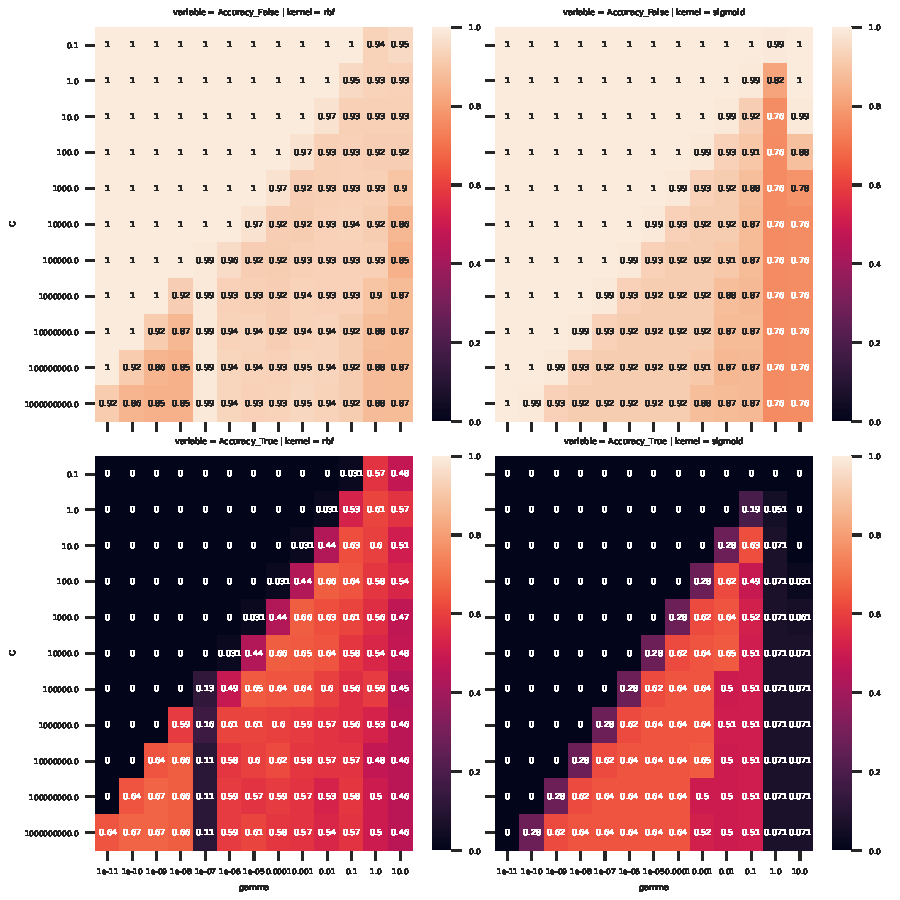
\includegraphics[width=.8\textwidth]{FinalProject/SVM_heat.pdf}
    \captionof{figure}{Exploration of SVM accuracy with different  hyper-parameters. Shown are the validation accuracies for classifying false alignments (top row) and true alignments (bottom row) across different choices for the hyper-parameters  $C$, $\gamma$, and two kernels "sigmoid," and "radial basis function (RBF)." }
    \label{fig:SVM}
\end{center}

I also tested a random forest classifier on the data. The random forest classifier performed better without hyper-parameter tuning than the SVM; however I found that the random forest model was less adjustable with respect to the hyper-parameters (\autoref{fig:RF}). I varied three major hyper-parameters to come to these conclusions: the number of trees used, the maximum number of features used at the decision points, and the minimum number of samples at each leaf in the tree. This is not close to an exhaustive set of hyper-parameters for random forest, so more exploration could be done, however these initial results indicate that random forest will probably not be the best classifier for the data. 

Finally I tried a gradient boosting classifier.  \autoref{fig:GB} shows validation accuracy while varying the following hyper-parameters: the learning rate which controls the contribution of each tree, and the number of trees used. Additionally I tried using two different loss functions: logistic loss, and exponential loss (i.e. AdaBoost loss \parencite{Freund1997ABoosting}). This classifier seems to be a good combination of the flexibility of SVM and stability of random forest for my data; however, just like random forest I have only explored a small portion of the hyper-parameter space so much more could be tested. 

My code for this project can be found at: \\
\texttt{https://github.com/mvollger/CSE546/tree/master/FinalProject}


\begin{center}
    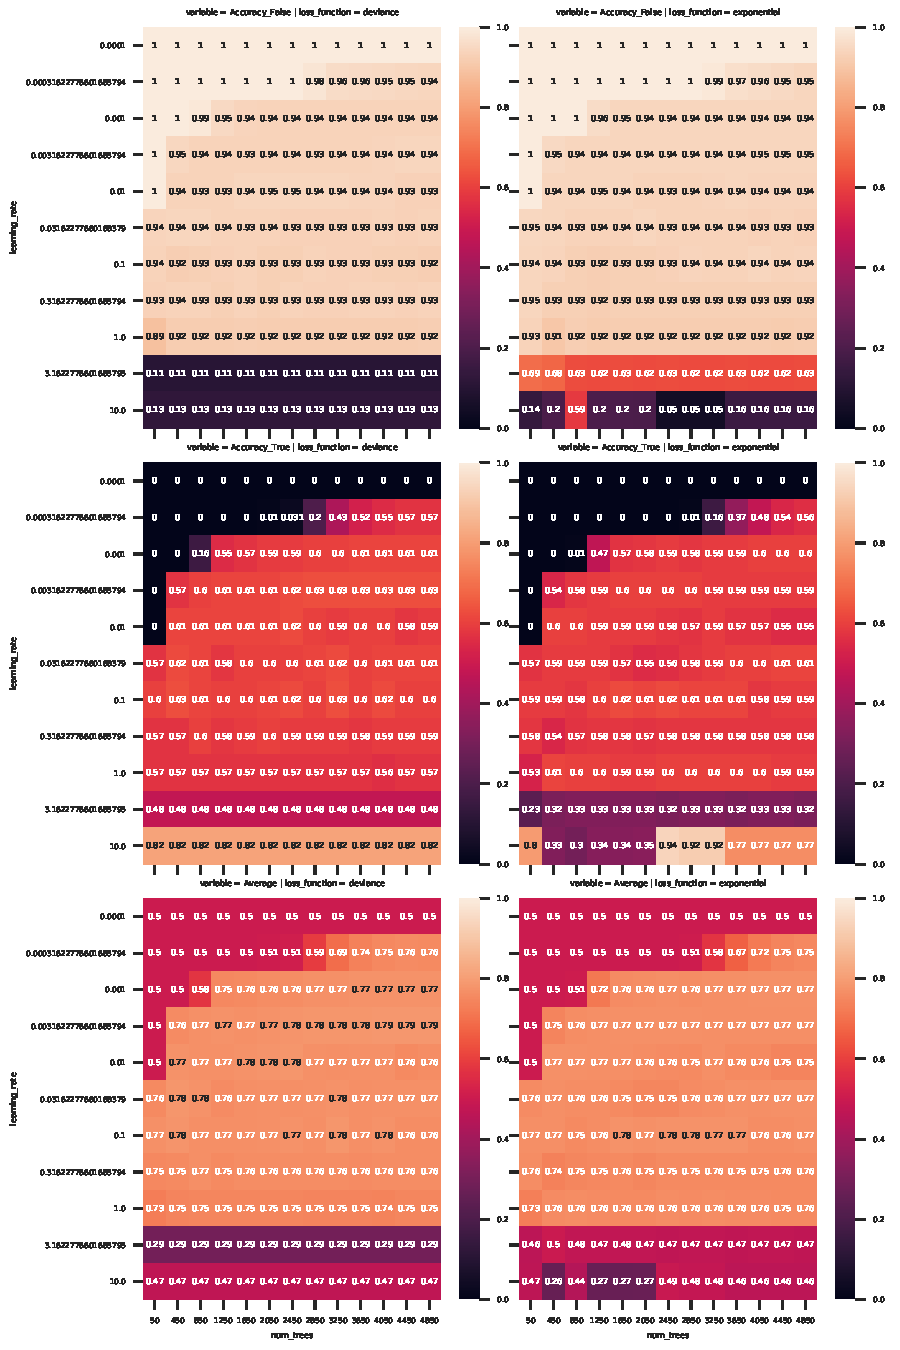
\includegraphics[width=0.8\textwidth]{FinalProject/GB_heat.pdf}
    \captionof{figure}{Exploration of Gradient boosting accuracy with different hyper-parameters. Shown are the validation accuracies for classifying false alignments (top row) and true alignments (bottom row) across different choices for the hyper-parameters  learning rate, number of trees, and two loss functions "deviance," and "exponential."}
    \label{fig:GB}
\end{center}



\section*{Final Project Goals}

I am interested in methods that can extract features from the raw alignments themselves instead of using summary statistics like percent identity, quality score, etc. For example, visualizations of alignments have been used to classify structural variants using convolutional neural nets. To take advantage of this additional dimension of my data I will use a "bag of words" approach to create extra features for my data. Alignments between a reference and query sequence are defined using a set of characters: "X" represents a mismatched position, "=" Represents a match, "D" represents a deletion in the query sequence, and finally "I" represents an insertion in the query sequence. Using this alphabet I will make every possible combination of 6 characters and the count the occurrences of each of the 6-mer in my data, to add addition features to each alignment. After adding these additional features to the data I will re-apply the techniques I have already described above as well as more completely explore the hyper-parameter space of each model.

Time permitting I plan to write my own implementation of the most successful classifier. One part of this will be implementing a modified loss function that penalizes miss-classified true alignments more than miss-classified false alignments, to encourage better classification of true alignments at the cost of sensitivity. This would serve as a way to combat the imbalance in the data set. In addition, I will experiment with selectively sub-sampling my training set to contain an equal number of true and false alignments. 

If I fail to improve the classification accuracy of true alignments using the strategies described above I will explore additional classification methods, e.g. convolution neural net, Gaussian process classification. 

%%%
%%%  REFERENCES
%%%
\printbibliography 


\beginsupplement

\section*{Appendix}


\begin{center}
    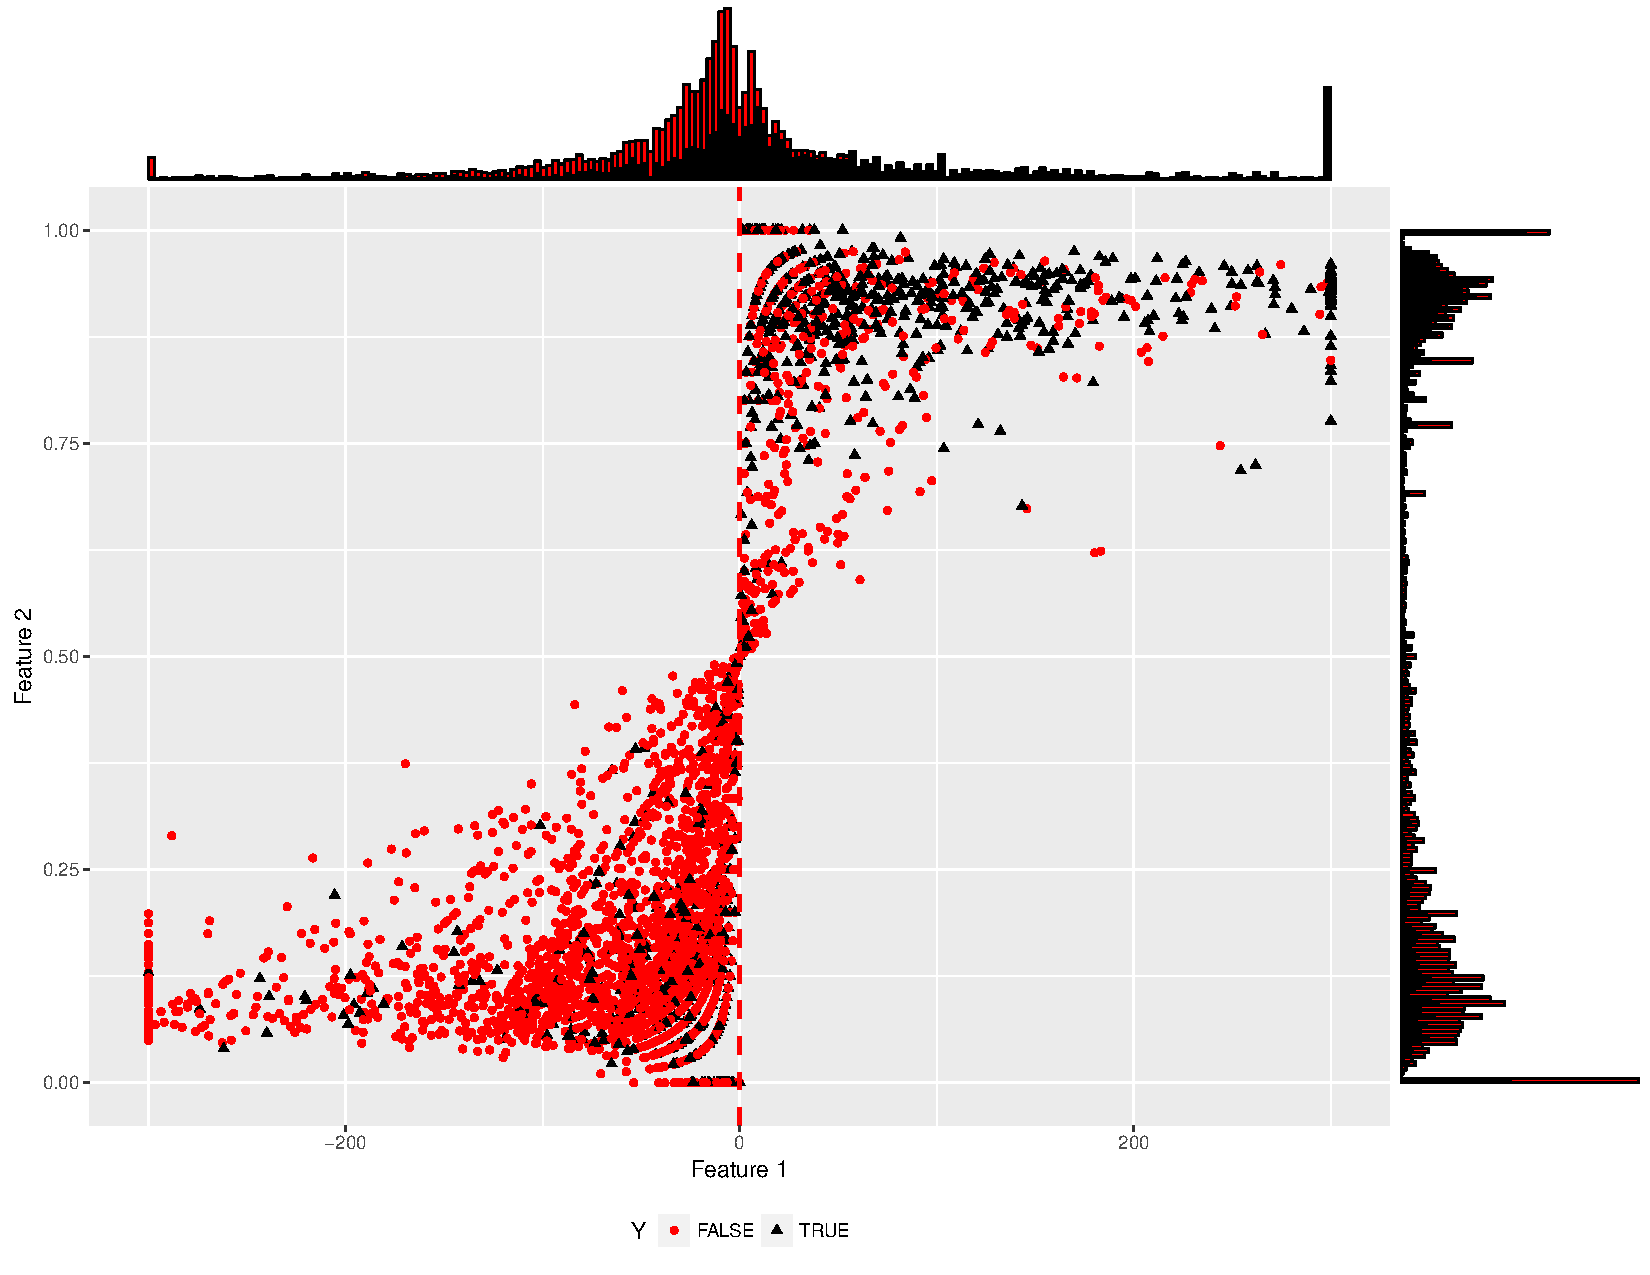
\includegraphics[width=0.8\textwidth]{FinalProject/LHRbyFRAC.pdf}
    \captionof{figure}{Two features of the data. Black indicates "true" alignments and "red" indicates false alignemnts.}
    \label{fig:LHR}
\end{center}


\begin{center}
    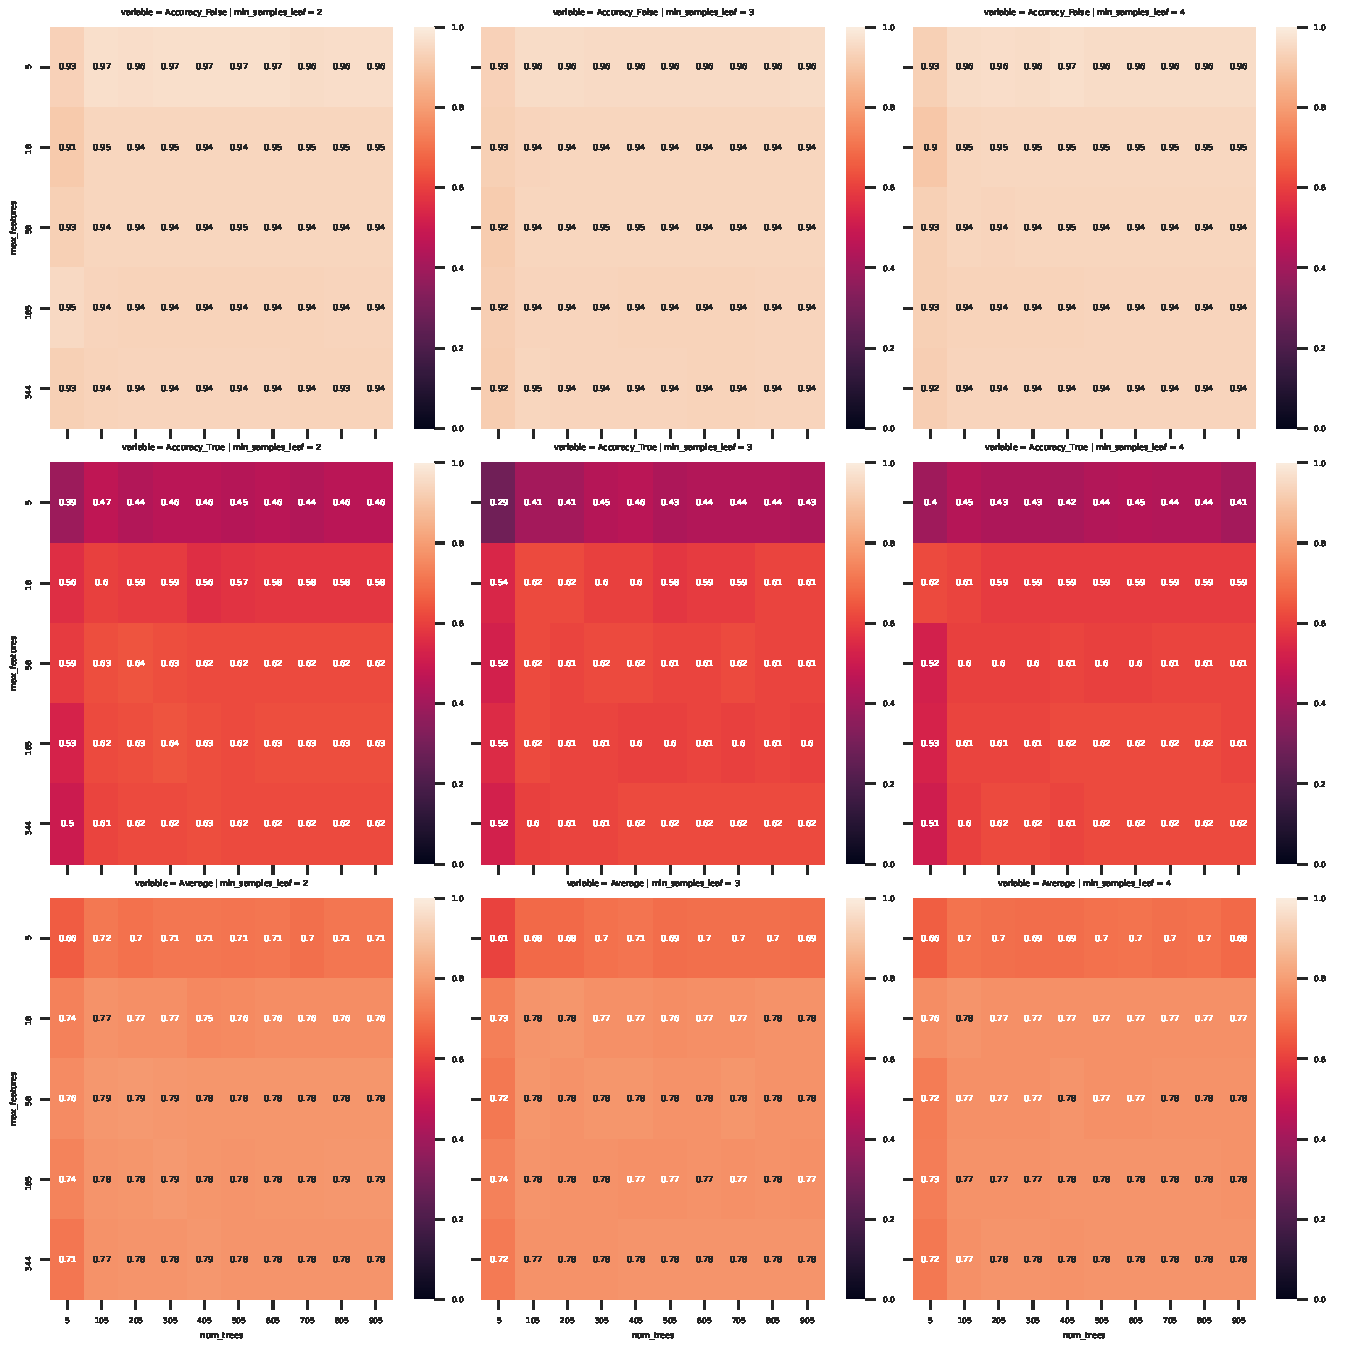
\includegraphics[width=0.8\textwidth]{FinalProject/RF_heat.pdf}
    \captionof{figure}{Exploration of Random Forest accuracy with different hyper-parameters.}
    \label{fig:RF}
\end{center}


\end{document}
